\documentclass[12pt]{article}

\input{../Tex/header.tex}
%\geometry{twoside,bindingoffset = 2cm,left = 15mm, right = 15mm}
\onehalfspacing
\renewcommand{\bibname}{References}
% opening
\title{Cylindrical shapes}
\author[1,2]{Samuel Richard Harrison}
\author[2]{\authorcr Supervisors: Prof. D.T. Papageorgiou}

\affil[1]{ University of Reading}
\affil[2]{Imperial College London}
\date{\today}

\begin{document}

\maketitle

\begin{abstract}
	Here I am going to look at how various periodic shapes affect the fluid dynamics
\end{abstract}

\section{Governing Equations}
Starting with a solid of radius $\tilde R(\tilde z,\tilde t)$, with a fluid flowing down it of thickness $a=a(\tilde z,\tilde t)$, assuming the system is axisymmetric.
\begin{figure}[H]
	\centering
	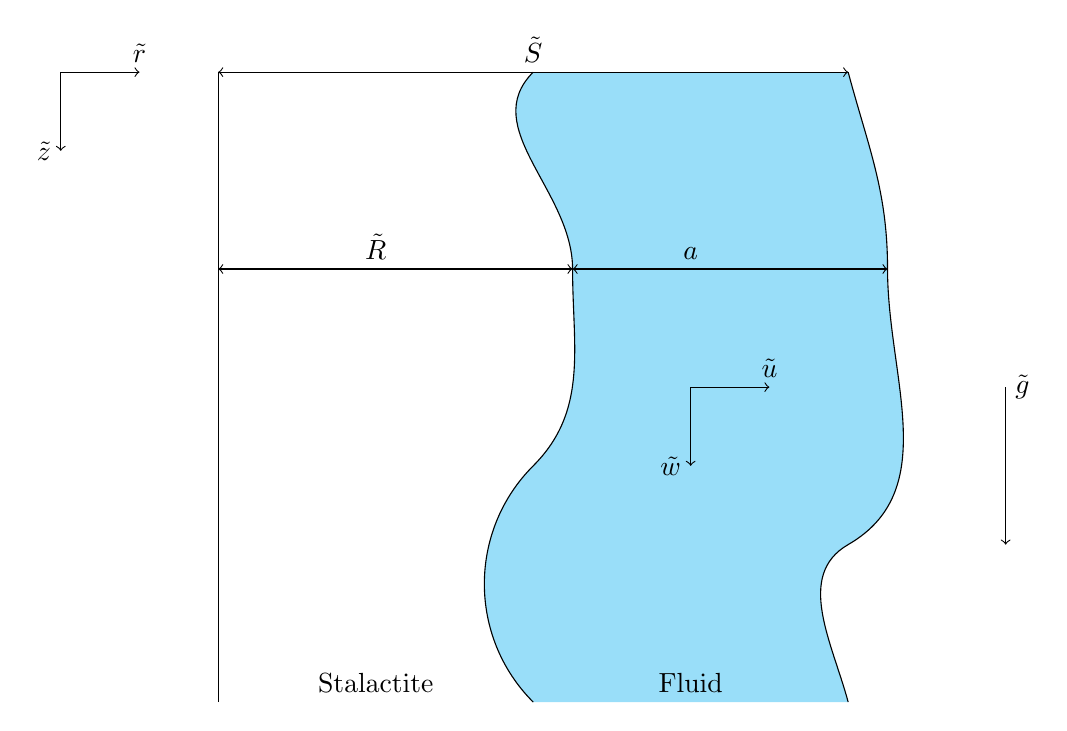
\begin{tikzpicture}
	\draw (0,0) -- (0,8);
	\fill[cyan!40!white] (4,0) to [out=135, in=-135] (4,3) to [out=45,in=-90]  (4.5,5.5) to [out=90,in=-135] (4,8) to (8,8) to [out=-75,in=90] (8.5,5.5) to [out=-90,in=30] (8,2) to [out=-150,in=105] (8,0) -- cycle;
	
	\draw (4,0) to [out=135, in=-135] (4,3) to [out=45,in=-90]  (4.5,5.5) to [out=90,in=-135] (4,8);
	\draw (8,0) to [out=105, in=-150] (8,2) to [out=30,in=-90]  (8.5,5.5) to [out=90,in=-75] (8,8);
	\draw[<->](0,5.5)--(4.5,5.5);
	\node[above] at (2,5.5) {$\tilde R$};
	\draw[<->](4.5,5.5)--(8.5,5.5);
	\node[above] at (6,5.5) {$a$};
	
	\draw[->] (6,4) --(6,3);
	\node[ left] at (6,3) {$\tilde w$};
	\draw[->] (6,4) --(7,4);
	\node[above ] at (7,4) {$\tilde u$};
	\draw[->] (10,4) --(10,2);
	\node[right] at (10,4) {$\tilde g$};
	\draw[<->] (0,8)--(8,8);
	\node[above] at (4,8) {$\tilde S$};
	\node[above] at (2,0) {Stalactite};
	\node[above] at (6,0) {Fluid};
	\draw[->] (-2,8) --(-2,7);
	\node[left] at (-2,7) {$\tilde z$};
	\draw[->] (-2,8) --(-1,8);
	\node[above] at (-1,8) {$\tilde r$};
	\end{tikzpicture}
	\caption{Geometry of the problem\label{fig:base_stalac}}
\end{figure}
For an incompressible fluid with velocity $\vec{\tilde u}=(\tilde u,0,\tilde w)$ in cylindrical coordinates $\vec{\tilde x}=(\tilde r,\tilde \theta,\tilde z)$. The continuity equation is
\begin{align}
\pdv{\tilde u}{\tilde r}+\frac{\tilde u}{\tilde r}+\pdv{\tilde w}{\tilde z}=0 \label{continuity}
\end{align}
And the Navier Stokes Equations give
\begin{align}
\pdv{\tilde u}{\tilde t}+\tilde u\pdv{\tilde u}{\tilde r}+\tilde w\pdv{\tilde u}{\tilde z}&=-\frac{1}{\rho}\pdv{\tilde p}{\tilde r}+\nu\left(\pdv[2]{\tilde u}{\tilde r}+\frac{1}{\tilde r}\pdv{\tilde u}{\tilde r}-\frac{1}{r^2}\tilde u+\pdv[2]{\tilde u}{\tilde z}\right)\label{navierr}\\
\pdv{\tilde w}{\tilde t}+u\pdv{\tilde w}{\tilde r}+\tilde w\pdv{\tilde w}{\tilde z}&=-\frac{1}{\rho}\pdv{\tilde p}{\tilde z}+\nu\left(\pdv[2]{\tilde w}{\tilde r}+\frac{1}{\tilde r}\pdv{\tilde w}{\tilde r}+\pdv[2]{\tilde w}{\tilde z}\right) + g \label{navierv}
\end{align}
On the boundary between the solid and the fluid we have no flux and no slip i.e
\begin{align}
\tilde u=0,\;\tilde  w=0\quad\mathrm{on}\; \tilde r=\tilde R \label{solidboundary}
\end{align}
On the surface of the fluid at $\tilde r=\tilde R+a=\tilde S(\tilde z,\tilde t)$, the kinematic boundary condition gives
\begin{align}
\tilde   u=\pdv{\tilde S}{\tilde t}+\tilde w\pdv{\tilde S}{\tilde z} \quad\mathrm{on}\;\tilde  r=\tilde S \label{kinematic}
\end{align}
The tangential and normal stress balances on the free surface gives
\footnotesize
\begin{align}
2\pdv{\tilde S}{\tilde z}\left(\pdv{\tilde u}{\tilde r}-\pdv{\tilde w}{\tilde z}\right)+\left(1-\left(\pdv{\tilde S}{\tilde z}\right)^2\right)\left(\pdv{\tilde u}{\tilde z}+\pdv{\tilde w}{\tilde r}\right)&=0\label{tangstress}\\
\tilde p\left(1+\left(\pdv{\tilde S}{\tilde z}\right)^2\right)-2\mu\left( \pdv{\tilde u}{\tilde r}-\pdv{\tilde S}{\tilde z}\left(\pdv{\tilde u}{\tilde z}+\pdv{\tilde w}{\tilde r}\right)+\left(\pdv{\tilde S}{\tilde z}\right)^2\pdv{\tilde w}{\tilde z}\right)&=\gamma\frac{\left(\frac{1}{\tilde S}\left(1+\left(\pdv{\tilde S}{\tilde z}\right)^2\right)-\pdv[2]{\tilde S}{\tilde z}\right)}{\left(1+\left(\pdv{\tilde S}{\tilde z}\right)^2\right)^{\frac{1}{2}}}\label{normstress}
\end{align}
\normalsize
at $\tilde r= \tilde{S}$
\subsection{Scaling}
Introduce non-dimensional variables

\begin{align}
(\tilde{r},\tilde{z},\tilde{R}, \tilde{S}, \tilde{a}) = a_0(r,z,R,S,a),\quad (\tilde{u},\tilde{v}) = \frac{a_0^2  g}{\nu}(u,v),\quad \tilde p=\rho  a_0g  p, \quad t=\frac{\nu}{a_0g}t
\end{align}
where $a_0$ is the mean fluid thickness.
This leads to 

\begin{align}
\pdv{ u}{ r}+\frac{ u}{ r}+\pdv{ w}{ z}=0 \label{continuityn}
\end{align}

\begin{align}
\Re\left(\pdv{ u}{ t}+ u\pdv{ u}{ r}+ w\pdv{ u}{ z}\right)&=-\pdv{ p}{ r}+\pdv[2]{ u}{ r}+\frac{1}{ r}\pdv{ u}{ r}-\frac{1}{r^2} u+\pdv[2]{ u}{ z}\label{navierrn}\\
\Re\left(\pdv{ w}{ t}+u\pdv{ w}{ r}+ w\pdv{ w}{ z}\right)&=-\pdv{ p}{ z}+\pdv[2]{ w}{ r}+\frac{1}{ r}\pdv{ w}{ r}+\pdv[2]{ w}{ z}+ 1 \label{naviervn}
\end{align}
where the Reynold's number, $\Re=\frac{a_0^3 g}{\nu^2}$. We are going to assume that $\Re\ll 1$, which leaves us with Stokes Flow. With Boundary conditions 

\begin{align}
 u=0,\;  w=0\quad\mathrm{on}\;  r= R \label{solidboundaryn}
\end{align}
\begin{align}
   u=\pdv{ S}{ t}+ w\pdv{ S}{ z} \quad\mathrm{on}\;  r= a + R =S \label{kinematicn}
\end{align}
The tangential and normal stress balances on the free surface gives
\footnotesize
\begin{align}
2\pdv{ S}{ z}\left(\pdv{ u}{ r}-\pdv{ w}{ z}\right)+\left(1-\left(\pdv{ S}{ z}\right)^2\right)\left(\pdv{ u}{ z}+\pdv{ w}{ r}\right)&=0\label{tangstressn}\\
 p\left(1+\left(\pdv{ S}{ z}\right)^2\right)-2\mu\left( \pdv{ u}{ r}-\pdv{ S}{ z}\left(\pdv{ u}{ z}+\pdv{ w}{ r}\right)+\left(\pdv{ S}{ z}\right)^2\pdv{ w}{ z}\right)&=\scr{B}\frac{\left(\frac{1}{ S}\left(1+\left(\pdv{ S}{ z}\right)^2\right)-\pdv[2]{ S}{ z}\right)}{\left(1+\left(\pdv{ S}{ z}\right)^2\right)^{\frac{1}{2}}}\label{normstressn}
\end{align}
\normalsize
at $ r= S$, where $\scr{B}=\Bo^{-1}$ is an inverted Bond number $\Bo =\frac{\rho a_0^2 g}{\gamma}.$
\section{Linear Analysis}
If we look at wall disturbances as a small perturbation to the cylindrical case we can write.

\begin{align}
u&=U(r)+\delta \tilde u(r,z)\label{eq:perturbtop}\\
w&=W(r)+\delta\tilde w(r,z)\\
p&=P(r)+\delta\tilde p(r,z)\\
\end{align}
With the fluid now in the region
\begin{align}
R+\delta\tilde r(z)\leq r\leq 1+R+\delta (\tilde s(z) \label{eq:perturbbottom}
\end{align}

\begin{figure}[H]
	\centering
	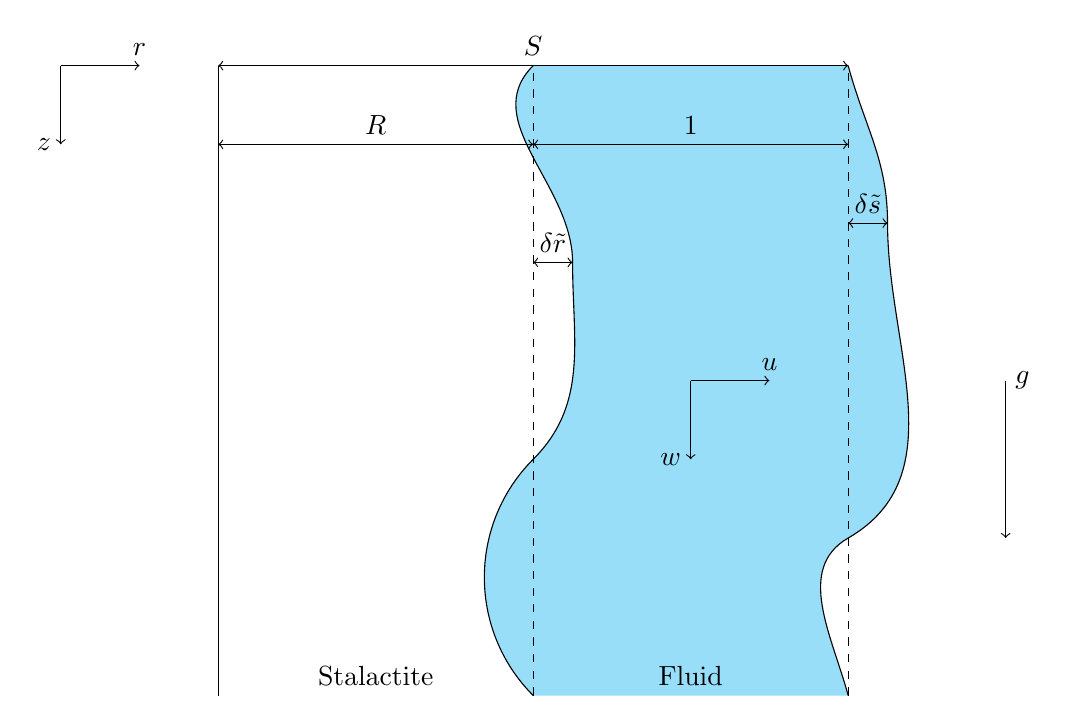
\begin{tikzpicture}
	\draw (0,0) -- (0,8);
	\fill[cyan!40!white] (4,0) to [out=135, in=-135] (4,3) to [out=45,in=-90]  (4.5,5.5) to [out=90,in=-135] (4,8) to (8,8) to [out=-75,in=90] (8.5,6) to [out=-90,in=30] (8,2) to [out=-150,in=105] (8,0) -- cycle;
	\draw[dashed](4,0) -- (4,8);
	\draw[dashed](8,0)--(8,8);
	\draw (4,0) to [out=135, in=-135] (4,3) to [out=45,in=-90]  (4.5,5.5) to [out=90,in=-135] (4,8);
	\draw (8,0) to [out=105, in=-150] (8,2) to [out=30,in=-90]  (8.5,6) to [out=90,in=-75] (8,8);
	\draw[<->](4,5.5)--(4.5,5.5);
	\node[above] at (4.25,5.5) {$\delta\tilde r$};
	\draw[<->](8,6)--(8.5,6);
	\node[above] at (8.25,6) {$\delta \tilde s$};
	\draw[<->] (0,7) --(4,7); 
	\node[above] at (2,7) {$R$};
	\draw[<->] (4,7) -- (8,7);
	\node[above] at (6,7) {$1$};
	\draw[->] (6,4) --(6,3);
	\node[ left] at (6,3) {$w$};
	\draw[->] (6,4) --(7,4);
	\node[above ] at (7,4) {$ u$};
	\draw[->] (10,4) --(10,2);
	\node[right] at (10,4) {$ g$};
	\draw[<->] (0,8)--(8,8);
	\node[above] at (4,8) {$ S$};
	\node[above] at (2,0) {Stalactite};
	\node[above] at (6,0) {Fluid};
	\draw[->] (-2,8) --(-2,7);
	\node[left] at (-2,7) {$ z$};
	\draw[->] (-2,8) --(-1,8);
	\node[above] at (-1,8) {$ r$};
	\end{tikzpicture}
	\caption{Stalactite with Crenulations\label{sta_cren}}
\end{figure}

Looking at the $O(1)$ terms, we find that
\begin{align}
U&=0\label{baseu1}\\
W&=\frac{1}{4}\left(R^2-r^2+2(1+R)^2\log\left(\frac{r}{R}\right)\right)\label{basew1}\\
P&=\frac{1}{\Bo S}\label{basep1}
\end{align}
Looking at the $O(\delta)$ terms we get 
\begin{align}
\frac{1}{r}\pdv{r}\left(r\tilde u\right)+\pdv{\tilde w}{z}&=0\label{smallconttop}\\
\frac{1}{r}\pdv{r}\left(r\pdv{\tilde u}{r}\right)-\frac{1}{r^2}\tilde u+\pdv[2]{\tilde u}{z}&=\pdv{\tilde p}{r}\\
\frac{1}{r}\pdv{r}\left(r\pdv{\tilde w}{r}\right)+\pdv[2]{\tilde w}{z}&=\pdv{\tilde p}{z}\label{smallcontbottom}
\end{align}
with boundary conditions
\begin{align}
\eval{\tilde u}_R&=0\label{boundarytop}\\
\eval{\tilde w}_R&= \left(\frac{1}{2R} +1\right)\tilde r\\
\eval{\tilde u}_{1+R}&=\frac{1}{4}\left(-1-2R+2(1+R)^2\log\left(\frac{1+R}{R}\right)\right)\dv{\tilde s}{z}\\
\eval{\pdv{\tilde u}{z}}_{1+R}+\eval{\pdv{\tilde w}{r}}_{1+R}&=\tilde s\\
\Bo\left(\eval{\tilde p}_{1+R}-2\eval{\pdv{\tilde u}{r}}_{1+R}\right)&=-\left(\frac{\tilde s}{(1+R)^2}+\dv[2]{\tilde s}{z}\right)\label{boundarybottom}
\end{align}

\end{document}          
